\section{Preconditioning}

\begin{tmp}
      Here we need to say general words about how we need an efficient preconditioning scheme.
\end{tmp}

\subsection{Preconditioning 101}

\subsection{Cholesky preconditioning for classical graphs}

\subsection{Classical collapsibility}

% TODO: introduction


In this section we borrow the terminology from \cite{whiteheadSimplicialSpacesNuclei1939}; additionally, let us  assume that considered simplicial complex \( \mc K \) is restricted to its \(2\)-skeleton, so \( \mc K \) consists only of nodes, edges, and triangles, \( \mc K = \V 0 \cup \V 1 \cup \V 2\).

Simplex \( \tau \in \mc K \) is called an (inlusion-wise) \gls{maximal face} of simplex \( \sigma \in \mc K \) if \( \tau \) is maximal by inlusion simplex such that \( \sigma \subseteq \tau \) and \( \ord \sigma < \ord \tau \). \en{
      \insidefigure[0.3\columnwidth]{\begin{tikzpicture}

      \fill [opacity=0.5,liberty]    (0, 0) -- (2, 0) --  (1, 1.5) -- cycle;
      \fill [opacity=0.3,liberty]    (0, 0) -- (2, 0) --  (1, -1.5) -- cycle;

      \Vertex[x=0, y=0, style={color=persimmon}, fontcolor=white, size=0.2, label = 1]{v1}
      \Vertex[x=2, y=0, style={color=persimmon}, fontcolor=white, size=0.2, label = 2]{v2}
      \Vertex[x=1, y=1.5, style={color=persimmon}, fontcolor=white, size=0.2, label = 3]{v3}
      \Vertex[x=1, y=-1.5, style={color=persimmon}, fontcolor=white, size=0.2, label = 4]{v4}

      \Edge[](v1)(v2)
      \Edge[](v1)(v3)
      \Edge[](v2)(v3)
      \Edge[](v1)(v4)
      \Edge[](v2)(v4)


\end{tikzpicture}}{Example of a simplicial complex: free simplices and maximal faces. \label{fig:adjacent_triangles}}
} For instance, in \Cref{fig:adjacent_triangles} the edge \( \{1, 2\} \) and nodes \( \{ 1 \} \) and \( \{ 2 \} \) have two maximal faces, \( \{ 1, 2, 3 \} \) and \( \{ 1, 2, 4 \} \), while all the other edges and nodes have unique maximal faces --- their corresponding triangles. Note that in the case of the node \( \{ 1 \} \), there are bigger simplices containing it besides the triangles (e.g. the edge \( \{ 1, 2 \} \)), but they are not maximal by inclusion.

\begin{definition}[Free simplex]\label{def:free}
      The simplex \(\sigma \in \mc K \) is \gls{free} if it has exactly one maximal face \( \tau \), \( \tau = \tau(\sigma) \). F.i. edges \( \{ 1, 3 \} \), \( \{ 1, 4 \} \), \( \{ 2, 3 \} \) and \( \{ 2, 4 \} \) are all free in \Cref{fig:adjacent_triangles}.
\end{definition} 

 The \gls{collapse} \( \mc K \backslash \{ \sigma \} \) of \( \mc K \) at a free simplex \( \sigma \) is the transition from the original simplicial complex \( \mc K \) to a smaller simplicial complex \( \mc L \) without the free simplex \( \sigma \) and the corresponding maximal face \( \tau \), \( \mc K \to \mc K' = \mc K - \sigma - \tau \); namely, one can eliminate a simplex \( \tau \) if it has an accessible (not included in another simplex) face \(\sigma\).

Naturally, one can perform several consequent collapses at  \( \Sigma = \{ \sigma_1, \sigma_2, \ldots \} \) assuming \( \sigma_i \) is free in collapse simplicial complex from the previous stage; \( \Sigma \) is called the \gls{collapsing sequence}. Formally:
 \begin{definition}[Collapsing sequence]
       Let \( \mc K \) be a simplicial complex. \( \Sigma = \{ \sigma_1, \sigma_2, \ldots \} \) is a \gls{collapsing sequence} if \( \sigma_1 \) is free in \( \mc K \) and each \( \sigma_i \), \( i > 1 \), is free at 
       \( \mc K^{(i)} = \mc K^{(i-1)} \backslash \{ \sigma_i \} \), \( \mc K^{(1)} = \mc K \). The collapse of \( \mc K \) to a new complex \( \mc L \) at \( \Sigma \) is denoted by \( \mc L = \mc K \backslash \Sigma \).
 \end{definition}
 By the definition, every collapsing sequence \( \Sigma \) has a corresponding sequence \( \ds T = \{ \tau(\sigma_1), \tau(\sigma_2), \ldots \} \) of maximal faces being collapsed at every step.

 \begin{definition}[Collapsible simplicial complex, \cite{whiteheadSimplicialSpacesNuclei1939}]
      The simplicial complex \( \mc K \) is \gls{collapsible} if there exists a collapsing sequence \( \Sigma \) such that \( \mc K \) collapses to a single vertex at \( \Sigma \), \( \mc K \backslash \Sigma = \{ v \} \).
\end{definition}

Determining whether the complex is collapsible is in general \emph{NP-complete},~\cite{tancerRecognitionCollapsibleComplexes2016}, but can be almost linear for a set of specific families of \( \mc K \), e.g.\ if the simplex can be embeded into the triangulation of the \(d\)-dimensional unit sphere,~\cite{cohenSolving1laplaciansNearly2014}. Naturally restricting the collapses to the case of \(d\)-collapses (such that \( \ord \sigma_i \le d-1 \)), one arrive at the notion of \(d\)-collapsibility,~\cite{tancerDcollapsibilityNPcomplete2009}.

\begin{definition}[\(d\)-Core]
      A \(d\)-Core is a subcomplex of \( \mc K \) such that every simplex of order \( d - 1\) belongs to at least \( 2 \) simplices of order \( d \). E.g. \(2\)-Core is such a subcomplex of the original 2-skeleton \( \mc K \) that every edge from \( \V 1 \) belong to at least \(2\) triangles from \( \V 2 \).
\end{definition}

\begin{lemma}[\cite{lofanoWorstWayCollapse2021}]
      \( \mc K \) is \(d\)-collapsible if and only if it does not contain a \( d\)-core.
\end{lemma}
\begin{proof}
      The proof of the lemma above naturally follows from the definition of the core. Assume \( \Sigma \) is a \(d\)-collapsing sequence, and \( \mc K \backslash \Sigma \) consists of more than a single vertex and has no free simplices of order \( \le d-1\) (``collapsing sequence gets stuck''). Then, each simplex of order \( d-1 \) is no free but belongs to at least \(2\) simplices of order \(d\), so \( \mc K \backslash \Sigma \) is a \( d \)-Core. Conversely if a \(d\)-Core exists in the complex, the collapsing sequence should necessarily include its \((d-1)\)-simplices which are not collapsible. %TODO : fix this
\end{proof}

In the case of the classical graph model, the \( 1 \)-Core is a subgraph where each vertex has a degree at least \( 2 \); in other words, \( 1 \)-Core cannot be a tree and necessarily contains a simple cycle. Hence, the collapsibility of a classical graph coincides with the acyclicity. The \(d\)-Core is the generalization of the cycle for the case of \(1\)-collapsibility of the classical graph; additionally, the \(d\)-Core is very dense due to its definition. In the case of \(2\)-Core, we provide simple exemplary structures on \Cref{fig:2-core} which imply various possible configurations for a  \(d\)-Core, \( d \ge 2 \), hence a search for \(d\)-Core inside \( \mc K \) is neither trivial, no computationally cheap.

\begin{figure}[htbp]
      \centering
      \begin{tikzpicture}
      \Vertex[x=0, y=0, size=0.25, fontscale=0.75, label=1]{v1}
      \Vertex[x=2, y=0, size=0.25, fontscale=0.75,label=2]{v2}
      \Vertex[x=1, y=1.5, size=0.25,fontscale=0.75, label=3]{v3}
      \Vertex[x=1, y=0.5, size=0.25,fontscale=0.75, label=4]{v4} 
      \Edge(v1)(v2)
      \Edge(v1)(v3)
      \Edge(v1)(v4)
      \Edge(v2)(v3)
      \Edge(v2)(v4)
      \Edge(v3)(v4)

      
      \Vertex[x=6, y=0, size=0.25, fontscale=0.75, label=1]{v1}
      \Vertex[x=5.5, y=1, size=0.25, fontscale=0.75, label=2]{v2}
      \Vertex[x=6.5, y=1, size=0.25, fontscale=0.75, label=3]{v3}
      \Vertex[x=4.25, y=-0.25, size=0.25, fontscale=0.75, label=4]{v4}
      \Vertex[x=7.75, y=-0.25, size=0.25, fontscale=0.75, label=5]{v5}
      \Vertex[x=6, y=2.25, size=0.25, fontscale=0.75, label=6]{v6}
      \Edge(v1)(v2)
      \Edge(v2)(v3)
      \Edge(v1)(v3)
      \Edge(v4)(v5)
      \Edge(v4)(v6)
      \Edge(v5)(v6)
      \Edge(v1)(v4)
      \Edge(v1)(v5)
      \Edge(v2)(v6)
      \Edge(v3)(v6)
      \Edge(v2)(v4)
      \Edge(v3)(v5)
\end{tikzpicture}
      \caption{ \(2\)-Core, examples. \label{fig:2-core} }
\end{figure}

%Besides the quantitative restriction discussed later, \( 2 \)-Cores tend to appear relatively early when upon ``densifying'' the complex.
Additionally, we demonstrate that an arbitrary simplicial complex \(\mc K\) tends to contain \(2\)-Cores as long as \( \mc K \) is denser than a trivially collapsible case. Assume the complex formed by triangulation of \( m_0 \) random points on the unit square with a sparsity pattern \( \nu \); the triangulation itself with the corresponding \( \nu_\Delta \) is collapsible, but a reasonably small addition of edges already creates a \(2\)-Core (since it is local), \Cref{fig:core_prob}, left. Similarly, sampled sensor networks, where \( \exists \sigma \in \V 1: \; \sigma = [v_1, v_2] \iff \| v_1 - v_2 \|_2 < \eps \) for a chosen percolation parameter \( \eps > 0 \), quickly form a 2-Core upon the densifying of the network.

\begin{figure}[htbp]
      \centering
      \scalebox{0.4}{
            % Recommended preamble:
% \usetikzlibrary{arrows.meta}
% \usetikzlibrary{backgrounds}
% \usepgfplotslibrary{patchplots}
% \usepgfplotslibrary{fillbetween}
% \pgfplotsset{%
%     layers/standard/.define layer set={%
%         background,axis background,axis grid,axis ticks,axis lines,axis tick labels,pre main,main,axis descriptions,axis foreground%
%     }{
%         grid style={/pgfplots/on layer=axis grid},%
%         tick style={/pgfplots/on layer=axis ticks},%
%         axis line style={/pgfplots/on layer=axis lines},%
%         label style={/pgfplots/on layer=axis descriptions},%
%         legend style={/pgfplots/on layer=axis descriptions},%
%         title style={/pgfplots/on layer=axis descriptions},%
%         colorbar style={/pgfplots/on layer=axis descriptions},%
%         ticklabel style={/pgfplots/on layer=axis tick labels},%
%         axis background@ style={/pgfplots/on layer=axis background},%
%         3d box foreground style={/pgfplots/on layer=axis foreground},%
%     },
% }

\begin{tikzpicture}[/tikz/background rectangle/.style={fill={rgb,1:red,1.0;green,1.0;blue,1.0}, draw opacity={1.0}}, show background rectangle]
      \begin{axis}[point meta max={nan}, point meta min={nan}, legend cell align={left}, legend columns={1}, title={}, title style={at={{(0.5,1)}}, anchor={south}, font={{\fontsize{18 pt}{23.400000000000002 pt}\selectfont}}, color={rgb,1:red,0.0;green,0.0;blue,0.0}, draw opacity={1.0}, rotate={0.0}, align={center}}, legend style={color={rgb,1:red,0.1333;green,0.1333;blue,0.3333}, draw opacity={0.1}, line width={1}, solid, fill={rgb,1:red,1.0;green,1.0;blue,1.0}, fill opacity={0.9}, text opacity={1.0}, font={{\fontsize{22 pt}{28.6 pt}\selectfont}}, text={rgb,1:red,0.0;green,0.0;blue,0.0}, cells={anchor={center}}, at={(0.98, 0.02)}, anchor={south east}}, axis background/.style={fill={rgb,1:red,1.0;green,1.0;blue,1.0}, opacity={1.0}}, anchor={north west}, xshift={1.0mm}, yshift={-1.0mm}, width={150.4mm}, height={150.4mm}, scaled x ticks={false}, xlabel={$\mathrm{sparsity \; (wrt \; triangulation)}$}, x tick style={draw={none}}, x tick label style={color={rgb,1:red,0.0;green,0.0;blue,0.0}, opacity={1.0}, rotate={0}}, xlabel style={at={(ticklabel cs:0.5)}, anchor=near ticklabel, at={{(ticklabel cs:0.5)}}, anchor={near ticklabel}, font={{\fontsize{22 pt}{28.6 pt}\selectfont}}, color={rgb,1:red,0.0;green,0.0;blue,0.0}, draw opacity={1.0}, rotate={0.0}}, xmode={log}, log basis x={10}, xmajorgrids={true}, xmin={0.993342357875681}, xmax={1.2577738078862484}, xticklabels={{$\nu_\Delta$,$1.1\nu_\Delta$,$1.25\nu_\Delta$}}, xtick={{1.0,1.1,1.25}}, xtick align={inside}, xticklabel style={font={{\fontsize{18 pt}{23.400000000000002 pt}\selectfont}}, color={rgb,1:red,0.0;green,0.0;blue,0.0}, draw opacity={1.0}, rotate={0.0}}, x grid style={color={rgb,1:red,0.1333;green,0.1333;blue,0.3333}, draw opacity={0.1}, line width={0.5}, solid}, extra x ticks={{}}, extra x tick labels={}, extra x tick style={grid={major}, x grid style={color={rgb,1:red,0.1333;green,0.1333;blue,0.3333}, draw opacity={0.05}, line width={0.5}, solid}, major tick length={0}}, x axis line style={{draw opacity = 0}}, scaled y ticks={false}, ylabel={$\mathrm{probability \; of \; 2-Core}$}, y tick style={draw={none}}, y tick label style={color={rgb,1:red,0.0;green,0.0;blue,0.0}, opacity={1.0}, rotate={0}}, ylabel style={at={(ticklabel cs:0.5)}, anchor=near ticklabel, at={{(ticklabel cs:0.5)}}, anchor={near ticklabel}, font={{\fontsize{22 pt}{28.6 pt}\selectfont}}, color={rgb,1:red,0.0;green,0.0;blue,0.0}, draw opacity={1.0}, rotate={0.0}}, ymode={log}, log basis y={10}, ymajorgrids={true}, ymin={0.23981602983131609}, ymax={1.0424657608411214}, yticklabels={{$0.25$,$0.5$,$1$}}, ytick={{0.25,0.5,1.0}}, ytick align={inside}, yticklabel style={font={{\fontsize{18 pt}{23.400000000000002 pt}\selectfont}}, color={rgb,1:red,0.0;green,0.0;blue,0.0}, draw opacity={1.0}, rotate={0.0}}, y grid style={color={rgb,1:red,0.1333;green,0.1333;blue,0.3333}, draw opacity={0.1}, line width={0.5}, solid}, extra y ticks={{}}, extra y tick labels={}, extra y tick style={grid={major}, y grid style={color={rgb,1:red,0.1333;green,0.1333;blue,0.3333}, draw opacity={0.05}, line width={0.5}, solid}, major tick length={0}}, y axis line style={{draw opacity = 0}}, colorbar={false}]
          \addplot[color={rgb,1:red,0.8;green,0.4;blue,0.4667}, name path={393a1deb-0ad5-49fa-841c-c2d680cf69bc}, draw opacity={1.0}, line width={1.2}, solid, mark={*}, mark size={4.5 pt}, mark repeat={1}, mark options={color={rgb,1:red,0.0;green,0.0;blue,0.0}, draw opacity={1.0}, fill={rgb,1:red,0.8;green,0.4;blue,0.4667}, fill opacity={1.0}, line width={0.0}, rotate={0}, solid}]
              table[row sep={\\}]
              {
                  \\
                  1.009246153846154  0.25  \\
                  1.0134923076923077  0.25  \\
                  1.0177384615384615  0.25  \\
                  1.0219846153846153  0.25  \\
                  1.0262307692307693  0.41  \\
                  1.030476923076923  0.41  \\
                  1.0347230769230769  0.41  \\
                  1.0389692307692306  0.558  \\
                  1.0432153846153847  0.558  \\
                  1.0474615384615384  0.558  \\
                  1.0517076923076922  0.558  \\
                  1.0559538461538462  0.674  \\
                  1.0602  0.674  \\
                  1.0644461538461538  0.674  \\
                  1.0686923076923076  0.674  \\
                  1.0729384615384616  0.758  \\
                  1.0771846153846154  0.758  \\
                  1.0814307692307692  0.758  \\
                  1.0856769230769232  0.846  \\
                  1.089923076923077  0.846  \\
                  1.0941692307692308  0.846  \\
                  1.0984153846153846  0.846  \\
                  1.1026615384615386  0.898  \\
                  1.1069076923076924  0.898  \\
                  1.1111538461538462  0.898  \\
                  1.1154  0.94  \\
                  1.119646153846154  0.94  \\
                  1.1238923076923077  0.94  \\
                  1.1281384615384615  0.94  \\
                  1.1323846153846155  0.958  \\
                  1.1366307692307693  0.958  \\
                  1.1408769230769231  0.958  \\
                  1.145123076923077  0.958  \\
                  1.149369230769231  0.974  \\
                  1.1536153846153847  0.974  \\
                  1.1578615384615385  0.974  \\
                  1.162107692307692  0.988  \\
                  1.166353846153846  0.988  \\
                  1.1705999999999999  0.988  \\
                  1.1748461538461537  0.988  \\
                  1.1790923076923077  0.994  \\
                  1.1833384615384615  0.994  \\
                  1.1875846153846152  0.994  \\
                  1.191830769230769  0.994  \\
                  1.196076923076923  0.998  \\
                  1.2003230769230768  0.998  \\
                  1.2045692307692306  0.998  \\
                  1.2088153846153846  1.0  \\
                  1.2130615384615384  1.0  \\
                  1.2173076923076922  1.0  \\
                  1.221553846153846  1.0  \\
                  1.2258  1.0  \\
                  1.2300461538461538  1.0  \\
                  1.2342923076923076  1.0  \\
                  1.2385384615384614  1.0  \\
                  1.2427846153846154  1.0  \\
                  1.2470307692307692  1.0  \\
              }
              ;
          \addlegendentry {$\mathcal{V}_0(\mathcal K)=24$}
          \addplot[color={rgb,1:red,0.2;green,0.1333;blue,0.5333}, name path={3388d577-df0a-4b0f-bb98-8e4a3883b6b4}, draw opacity={1.0}, line width={1.2}, solid, mark={*}, mark size={4.5 pt}, mark repeat={1}, mark options={color={rgb,1:red,0.0;green,0.0;blue,0.0}, draw opacity={1.0}, fill={rgb,1:red,0.2;green,0.1333;blue,0.5333}, fill opacity={1.0}, line width={0.0}, rotate={0}, solid}]
              table[row sep={\\}]
              {
                  \\
                  1.0153999999999999  0.476  \\
                  1.0179999999999998  0.476  \\
                  1.0206  0.476  \\
                  1.0231999999999999  0.476  \\
                  1.0257999999999998  0.476  \\
                  1.0283999999999998  0.476  \\
                  1.031  0.476  \\
                  1.0335999999999999  0.476  \\
                  1.0361999999999998  0.476  \\
                  1.0388  0.476  \\
                  1.0413999999999999  0.476  \\
                  1.0439999999999998  0.8  \\
                  1.0466  0.8  \\
                  1.0492  0.8  \\
                  1.0517999999999998  0.8  \\
                  1.0543999999999998  0.8  \\
                  1.057  0.8  \\
                  1.0595999999999999  0.8  \\
                  1.0621999999999998  0.8  \\
                  1.0648  0.8  \\
                  1.0674  0.8  \\
                  1.0699999999999998  0.8  \\
                  1.0726  0.916  \\
                  1.0752  0.916  \\
                  1.0777999999999999  0.916  \\
                  1.0803999999999998  0.916  \\
                  1.083  0.916  \\
                  1.0856  0.916  \\
                  1.0881999999999998  0.916  \\
                  1.0908  0.916  \\
                  1.0934  0.916  \\
                  1.0959999999999999  0.916  \\
                  1.0986  0.916  \\
                  1.1011999999999997  0.972  \\
                  1.1037999999999997  0.972  \\
                  1.1063999999999998  0.972  \\
                  1.1089999999999998  0.972  \\
                  1.1115999999999997  0.972  \\
                  1.1141999999999999  0.972  \\
                  1.1167999999999998  0.972  \\
                  1.1193999999999997  0.972  \\
                  1.1219999999999999  0.972  \\
                  1.1245999999999998  0.972  \\
                  1.1271999999999998  0.972  \\
                  1.1297999999999997  0.986  \\
                  1.1323999999999999  0.986  \\
                  1.1349999999999998  0.986  \\
                  1.1375999999999997  0.986  \\
                  1.1401999999999999  0.986  \\
                  1.1427999999999998  0.986  \\
                  1.1453999999999998  0.986  \\
                  1.148  0.986  \\
                  1.1505999999999998  0.986  \\
                  1.1531999999999998  0.986  \\
                  1.1557999999999997  0.986  \\
                  1.1583999999999999  0.998  \\
                  1.1609999999999998  0.998  \\
                  1.1635999999999997  0.998  \\
                  1.1662  0.998  \\
                  1.1687999999999998  0.998  \\
                  1.1713999999999998  0.998  \\
                  1.174  0.998  \\
                  1.1765999999999999  0.998  \\
                  1.1791999999999998  0.998  \\
                  1.1817999999999997  0.998  \\
                  1.1844  0.998  \\
                  1.1869999999999998  1.0  \\
                  1.1895999999999998  1.0  \\
                  1.1922  1.0  \\
                  1.1947999999999999  1.0  \\
                  1.1973999999999998  1.0  \\
                  1.2  1.0  \\
                  1.2026  1.0  \\
                  1.2051999999999998  1.0  \\
                  1.2077999999999998  1.0  \\
                  1.2104  1.0  \\
                  1.2129999999999999  1.0  \\
                  1.2155999999999998  1.0  \\
                  1.2182  1.0  \\
                  1.2207999999999999  1.0  \\
                  1.2233999999999998  1.0  \\
                  1.226  1.0  \\
                  1.2286  1.0  \\
                  1.2311999999999999  1.0  \\
                  1.2337999999999998  1.0  \\
                  1.2363999999999997  1.0  \\
                  1.2389999999999997  1.0  \\
                  1.2415999999999998  1.0  \\
                  1.2441999999999998  1.0  \\
                  1.2467999999999997  1.0  \\
                  1.2493999999999998  1.0  \\
              }
              ;
          \addlegendentry {$\mathcal{V}_0(\mathcal K)=14$}
          \addplot[color={rgb,1:red,0.8667;green,0.8;blue,0.4667}, name path={51c0f6ce-ed32-4088-b026-cb9827a330bb}, draw opacity={1.0}, line width={1.2}, solid, mark={*}, mark size={4.5 pt}, mark repeat={1}, mark options={color={rgb,1:red,0.0;green,0.0;blue,0.0}, draw opacity={1.0}, fill={rgb,1:red,0.8667;green,0.8;blue,0.4667}, fill opacity={1.0}, line width={0.0}, rotate={0}, solid}]
              table[row sep={\\}]
              {
                  \\
                  1.0118399999999999  0.33  \\
                  1.01526  0.33  \\
                  1.01868  0.33  \\
                  1.0221  0.33  \\
                  1.02552  0.33  \\
                  1.02894  0.33  \\
                  1.03236  0.556  \\
                  1.03578  0.556  \\
                  1.0392  0.556  \\
                  1.0426199999999999  0.556  \\
                  1.04604  0.556  \\
                  1.04946  0.556  \\
                  1.05288  0.706  \\
                  1.0563  0.706  \\
                  1.05972  0.706  \\
                  1.06314  0.706  \\
                  1.06656  0.706  \\
                  1.06998  0.706  \\
                  1.0734  0.812  \\
                  1.07682  0.812  \\
                  1.08024  0.812  \\
                  1.08366  0.812  \\
                  1.08708  0.812  \\
                  1.0905  0.892  \\
                  1.09392  0.892  \\
                  1.09734  0.892  \\
                  1.10076  0.892  \\
                  1.10418  0.892  \\
                  1.1076  0.892  \\
                  1.11102  0.934  \\
                  1.1144399999999999  0.934  \\
                  1.1178599999999999  0.934  \\
                  1.1212799999999998  0.934  \\
                  1.1246999999999998  0.934  \\
                  1.1281199999999998  0.934  \\
                  1.13154  0.964  \\
                  1.13496  0.964  \\
                  1.13838  0.964  \\
                  1.1418  0.964  \\
                  1.14522  0.964  \\
                  1.1486399999999999  0.964  \\
                  1.1520599999999999  0.982  \\
                  1.1554799999999998  0.982  \\
                  1.1588999999999998  0.982  \\
                  1.16232  0.982  \\
                  1.16574  0.982  \\
                  1.16916  0.982  \\
                  1.17258  0.99  \\
                  1.176  0.99  \\
                  1.17942  0.99  \\
                  1.18284  0.99  \\
                  1.1862599999999999  0.99  \\
                  1.1896799999999998  0.99  \\
                  1.1931  0.998  \\
                  1.19652  0.998  \\
                  1.19994  0.998  \\
                  1.20336  0.998  \\
                  1.20678  0.998  \\
                  1.2102  0.998  \\
                  1.21362  0.998  \\
                  1.21704  0.998  \\
                  1.2204599999999999  0.998  \\
                  1.22388  0.998  \\
                  1.2273  0.998  \\
                  1.23072  1.0  \\
                  1.23414  1.0  \\
                  1.23756  1.0  \\
                  1.24098  1.0  \\
                  1.2444  1.0  \\
                  1.24782  1.0  \\
              }
              ;
          \addlegendentry {$\mathcal{V}_0(\mathcal K)=19$}
          \addplot[color={rgb,1:red,0.0;green,0.0;blue,0.0}, name path={4ecd3d1f-f31e-4dfa-ab9c-f882761805cd}, draw opacity={1.0}, line width={1.2}, dashed, forget plot]
              table[row sep={\\}]
              {
                  \\
                  1.0  0.25  \\
                  1.0  1.0  \\
              }
              ;
      \end{axis}
      \end{tikzpicture}
      
      }%
      \scalebox{0.4}{
            % Recommended preamble:
% \usetikzlibrary{arrows.meta}
% \usetikzlibrary{backgrounds}
% \usepgfplotslibrary{patchplots}
% \usepgfplotslibrary{fillbetween}
% \pgfplotsset{%
%     layers/standard/.define layer set={%
%         background,axis background,axis grid,axis ticks,axis lines,axis tick labels,pre main,main,axis descriptions,axis foreground%
%     }{
%         grid style={/pgfplots/on layer=axis grid},%
%         tick style={/pgfplots/on layer=axis ticks},%
%         axis line style={/pgfplots/on layer=axis lines},%
%         label style={/pgfplots/on layer=axis descriptions},%
%         legend style={/pgfplots/on layer=axis descriptions},%
%         title style={/pgfplots/on layer=axis descriptions},%
%         colorbar style={/pgfplots/on layer=axis descriptions},%
%         ticklabel style={/pgfplots/on layer=axis tick labels},%
%         axis background@ style={/pgfplots/on layer=axis background},%
%         3d box foreground style={/pgfplots/on layer=axis foreground},%
%     },
% }

\begin{tikzpicture}[/tikz/background rectangle/.style={fill={rgb,1:red,1.0;green,1.0;blue,1.0}, draw opacity={1.0}}, show background rectangle]
      \begin{axis}[point meta max={nan}, point meta min={nan}, legend cell align={left}, legend columns={1}, title={}, title style={at={{(0.5,1)}}, anchor={south}, font={{\fontsize{18 pt}{23.400000000000002 pt}\selectfont}}, color={rgb,1:red,0.0;green,0.0;blue,0.0}, draw opacity={1.0}, rotate={0.0}, align={center}}, legend style={color={rgb,1:red,0.1333;green,0.1333;blue,0.3333}, draw opacity={0.1}, line width={1}, solid, fill={rgb,1:red,1.0;green,1.0;blue,1.0}, fill opacity={0.9}, text opacity={1.0}, font={{\fontsize{22 pt}{28.6 pt}\selectfont}}, text={rgb,1:red,0.0;green,0.0;blue,0.0}, cells={anchor={center}}, at={(0.98, 0.02)}, anchor={south east}}, axis background/.style={fill={rgb,1:red,1.0;green,1.0;blue,1.0}, opacity={1.0}}, anchor={north west}, xshift={1.0mm}, yshift={-1.0mm}, width={150.4mm}, height={150.4mm}, scaled x ticks={false}, xlabel={$\mathrm{percolation, \;} \varepsilon$}, x tick style={draw={none}}, x tick label style={color={rgb,1:red,0.0;green,0.0;blue,0.0}, opacity={1.0}, rotate={0}}, xlabel style={at={(ticklabel cs:0.5)}, anchor=near ticklabel, at={{(ticklabel cs:0.5)}}, anchor={near ticklabel}, font={{\fontsize{22 pt}{28.6 pt}\selectfont}}, color={rgb,1:red,0.0;green,0.0;blue,0.0}, draw opacity={1.0}, rotate={0.0}}, xmode={log}, log basis x={10}, xmajorgrids={true}, xmin={1.1861535216168422}, xmax={13.35992353529639}, xticklabels={{$\varepsilon_{\min}$,$3\varepsilon_{\min}$,$10\varepsilon_{\min}$}}, xtick={{1.2,3.0,10.0}}, xtick align={inside}, xticklabel style={font={{\fontsize{18 pt}{23.400000000000002 pt}\selectfont}}, color={rgb,1:red,0.0;green,0.0;blue,0.0}, draw opacity={1.0}, rotate={0.0}}, x grid style={color={rgb,1:red,0.1333;green,0.1333;blue,0.3333}, draw opacity={0.1}, line width={0.5}, solid}, extra x ticks={{}}, extra x tick labels={}, extra x tick style={grid={major}, x grid style={color={rgb,1:red,0.1333;green,0.1333;blue,0.3333}, draw opacity={0.05}, line width={0.5}, solid}, major tick length={0}}, x axis line style={{draw opacity = 0}}, scaled y ticks={false}, ylabel={$\mathrm{probability \; of \; 2-Core}$}, y tick style={draw={none}}, y tick label style={color={rgb,1:red,0.0;green,0.0;blue,0.0}, opacity={1.0}, rotate={0}}, ylabel style={at={(ticklabel cs:0.5)}, anchor=near ticklabel, at={{(ticklabel cs:0.5)}}, anchor={near ticklabel}, font={{\fontsize{22 pt}{28.6 pt}\selectfont}}, color={rgb,1:red,0.0;green,0.0;blue,0.0}, draw opacity={1.0}, rotate={0.0}}, ymode={log}, log basis y={10}, ymajorgrids={true}, ymin={0.0016598196262967637}, ymax={1.204950205620966}, yticklabels={{$0.01$,$0.10$,$1.00$}}, ytick={{0.01,0.1,1.0}}, ytick align={inside}, yticklabel style={font={{\fontsize{18 pt}{23.400000000000002 pt}\selectfont}}, color={rgb,1:red,0.0;green,0.0;blue,0.0}, draw opacity={1.0}, rotate={0.0}}, y grid style={color={rgb,1:red,0.1333;green,0.1333;blue,0.3333}, draw opacity={0.1}, line width={0.5}, solid}, extra y ticks={{0.002,0.003,0.004,0.005,0.006,0.007,0.008,0.009,0.020000000000000004,0.030000000000000006,0.04000000000000001,0.05000000000000001,0.06000000000000001,0.07,0.08000000000000002,0.09000000000000001,0.2,0.3,0.4,0.5,0.6,0.7,0.8,0.9}}, extra y tick labels={}, extra y tick style={grid={major}, y grid style={color={rgb,1:red,0.1333;green,0.1333;blue,0.3333}, draw opacity={0.05}, line width={0.5}, solid}, major tick length={0.1cm}}, y axis line style={{draw opacity = 0}}, colorbar={false}]
          \addplot[color={rgb,1:red,0.8;green,0.4;blue,0.4667}, name path={42c6205a-4cd9-4520-973d-f08c26442123}, draw opacity={1.0}, line width={1.2}, solid, mark={*}, mark size={4.5 pt}, mark repeat={1}, mark options={color={rgb,1:red,0.0;green,0.0;blue,0.0}, draw opacity={1.0}, fill={rgb,1:red,0.8;green,0.4;blue,0.4667}, fill opacity={1.0}, line width={0.0}, rotate={0}, solid}]
              table[row sep={\\}]
              {
                  \\
                  2.119510426926017  0.002  \\
                  2.3993880336575213  0.008  \\
                  2.679265640389026  0.01  \\
                  2.9591432471205303  0.02  \\
                  3.239020853852034  0.048  \\
                  3.518898460583539  0.09  \\
                  3.7987760673150435  0.138  \\
                  4.078653674046547  0.186  \\
                  4.358531280778052  0.238  \\
                  4.638408887509556  0.304  \\
                  4.918286494241061  0.374  \\
                  5.198164100972565  0.468  \\
                  5.478041707704069  0.556  \\
                  5.757919314435574  0.648  \\
                  6.037796921167077  0.74  \\
                  6.317674527898582  0.808  \\
                  6.597552134630086  0.86  \\
                  6.87742974136159  0.902  \\
                  7.157307348093094  0.93  \\
                  7.437184954824598  0.964  \\
                  7.717062561556103  0.984  \\
                  7.996940168287607  0.992  \\
                  8.276817775019111  0.996  \\
                  8.556695381750616  0.998  \\
                  8.836572988482121  1.0  \\
                  9.116450595213625  1.0  \\
                  9.39632820194513  1.0  \\
                  9.676205808676633  1.0  \\
                  9.956083415408138  1.0  \\
                  10.235961022139643  1.0  \\
                  10.515838628871148  1.0  \\
                  10.79571623560265  1.0  \\
                  11.075593842334154  1.0  \\
                  11.355471449065659  1.0  \\
                  11.635349055797164  1.0  \\
                  11.915226662528667  1.0  \\
                  12.195104269260172  1.0  \\
                  12.474981875991677  1.0  \\
              }
              ;
          \addlegendentry {$\mathcal{V}_0(\mathcal K) = 20$}
          \addplot[color={rgb,1:red,0.2;green,0.1333;blue,0.5333}, name path={967f48f7-b1c1-4ee6-b4f5-4cdd98b0715d}, draw opacity={1.0}, line width={1.2}, solid, mark={*}, mark size={4.5 pt}, mark repeat={1}, mark options={color={rgb,1:red,0.0;green,0.0;blue,0.0}, draw opacity={1.0}, fill={rgb,1:red,0.2;green,0.1333;blue,0.5333}, fill opacity={1.0}, line width={0.0}, rotate={0}, solid}]
              table[row sep={\\}]
              {
                  \\
                  1.2702960619462884  0.002  \\
                  1.4054440929194325  0.002  \\
                  1.5405921238925768  0.002  \\
                  1.675740154865721  0.002  \\
                  1.810888185838865  0.004  \\
                  1.9460362168120093  0.006  \\
                  2.081184247785153  0.01  \\
                  2.2163322787582977  0.018  \\
                  2.351480309731442  0.032  \\
                  2.486628340704586  0.04  \\
                  2.62177637167773  0.05  \\
                  2.756924402650874  0.068  \\
                  2.8920724336240187  0.084  \\
                  3.0272204645971628  0.116  \\
                  3.162368495570307  0.136  \\
                  3.297516526543451  0.166  \\
                  3.4326645575165955  0.182  \\
                  3.5678125884897396  0.21  \\
                  3.702960619462884  0.246  \\
                  3.838108650436028  0.278  \\
                  3.973256681409172  0.308  \\
                  4.108404712382316  0.358  \\
                  4.24355274335546  0.398  \\
                  4.378700774328604  0.436  \\
                  4.513848805301748  0.476  \\
                  4.648996836274892  0.52  \\
                  4.7841448672480364  0.57  \\
                  4.919292898221181  0.622  \\
                  5.0544409291943255  0.668  \\
                  5.18958896016747  0.724  \\
                  5.324736991140614  0.766  \\
                  5.459885022113759  0.802  \\
                  5.595033053086903  0.842  \\
                  5.730181084060047  0.872  \\
                  5.86532911503319  0.9  \\
                  6.000477146006334  0.918  \\
              }
              ;
          \addlegendentry {$\mathcal{V}_0(\mathcal K) = 10$}
          \addplot[color={rgb,1:red,0.8667;green,0.8;blue,0.4667}, name path={3411fdfb-e7e5-400f-bd2e-38bdf50c0d5f}, draw opacity={1.0}, line width={1.2}, solid, mark={*}, mark size={4.5 pt}, mark repeat={1}, mark options={color={rgb,1:red,0.0;green,0.0;blue,0.0}, draw opacity={1.0}, fill={rgb,1:red,0.8667;green,0.8;blue,0.4667}, fill opacity={1.0}, line width={0.0}, rotate={0}, solid}]
              table[row sep={\\}]
              {
                  \\
                  1.831715935088466  0.002  \\
                  2.0396449188605827  0.008  \\
                  2.247573902632699  0.01  \\
                  2.4555028864048154  0.014  \\
                  2.6634318701769324  0.024  \\
                  2.8713608539490485  0.046  \\
                  3.079289837721165  0.062  \\
                  3.2872188214932816  0.094  \\
                  3.4951478052653977  0.112  \\
                  3.7030767890375147  0.156  \\
                  3.9110057728096312  0.182  \\
                  4.118934756581747  0.224  \\
                  4.326863740353864  0.292  \\
                  4.534792724125981  0.346  \\
                  4.742721707898097  0.418  \\
                  4.950650691670213  0.48  \\
                  5.15857967544233  0.538  \\
                  5.366508659214446  0.618  \\
                  5.574437642986563  0.676  \\
                  5.782366626758679  0.736  \\
                  5.990295610530796  0.782  \\
                  6.198224594302913  0.838  \\
                  6.406153578075029  0.876  \\
                  6.614082561847146  0.91  \\
                  6.822011545619263  0.93  \\
                  7.029940529391379  0.946  \\
                  7.237869513163496  0.966  \\
                  7.445798496935612  0.98  \\
                  7.653727480707729  0.99  \\
                  7.861656464479846  0.992  \\
                  8.069585448251962  1.0  \\
                  8.277514432024079  1.0  \\
                  8.485443415796194  1.0  \\
                  8.693372399568311  1.0  \\
                  8.901301383340428  1.0  \\
                  9.109230367112545  1.0  \\
                  9.317159350884662  1.0  \\
              }
              ;
          \addlegendentry {$\mathcal{V}_0(\mathcal K) = 15$}
      \end{axis}
      \end{tikzpicture}
      
      }
      \caption{ The probability of the \( 2 \)-Core in richer-than-triangulation simplicial complexes: triangulation of random points modified to have \( \left[ \nu \frac{ | \V 0 | \cdot ( | \V 0 | - 1 ) }{2} \right] \) edges on the left; random sensor networks with \( \eps \)-percolation on the right. \( \nu_\Delta \) defines the initial sparsity of the triangulated network; \(\eps_{\min} = \ds E \min_{x, y \in [0, 1]^2} \| x - y\|_2 \) is the minimal possible percolation parameter. \label{fig:core_prob} }
\end{figure}

However, in the following, we observe that a weaker condition is enough to efficiently design a preconditioner for any ``sparse enough'' simplicial complex.

\subsection{Weak collapsibility}


Let the complex \( \mc K \) be restricted up to its \(2\)-skeleton, \( \mc K = \V 0 \cup \V 1 \cup \V 2 \), and \( \mc K \) is collapsible. Then the collapsing sequence \( \Sigma \) necessarily involves collapses at simplices \( \sigma_i \) of different orders: at edges (eliminating \emph{edges} and \emph{triangles}) and at vertices (eliminating \emph{vertices} and \emph{edges}). One can show that for a given collapsing sequence \( \Sigma \) there is a reordering \( \tilde \Sigma \) such that \( \dim \tilde{\sigma_i} \) are non-increasing, {\cite[Lemma 2.5]{cohenSolving1laplaciansNearly2014}}. Namely, if such a complex is collapsible, then there is a collapsible sequence \( \Sigma = \{ \Sigma_1, \Sigma_0 \} \) where \( \Sigma_1 \) contains all the collapses at edges first and \( \Sigma_0 \) is composed of collapses at vertices. Note that the partial collapse \( \mc K \backslash \Sigma_1 = \mc L \) eliminates all the triangles in the complex, \( \mc V_2 (\mc L) = \varnothing \); otherwise, the whole sequence \( \Sigma \) is not collapsing \( \mc K \) to a single vertex. Since \( \mc V_2 (\mc L ) = \varnothing \), the associated up-Laplacian \( \Lu 1 ( \mc L ) = 0 \).

\begin{definition}[Weakly collapsible complex]
      Simplicial complex \( \mc K \) restricted to its \(2\)-skeleton is called \emph{weakly collapsible}, if there exists a collapsing sequence \( \Sigma_1 \) such that the simplicial complex \( \mc L = \mc K \backslash \Sigma_1 \) has no simplices of order \(2\), \( \mc V_2(\mc L) = \varnothing \) and \( \Lu 1 (\mc L ) = 0 \).
\end{definition}

\begin{example}
      Note that a collapsible complex is necessarily weakly collapsible; the opposite does not hold. Consider the following example in \Cref{fig:weak_example}: the initial complex is weakly collapsible either by a collapse at \( [3, 4] \) or at \( [2, 4] \). After this, the only available collapse is at the vertex \([4]\) leaving the uncollapsible \(3\)-vertex structure.
      \insidefigure[\columnwidth]{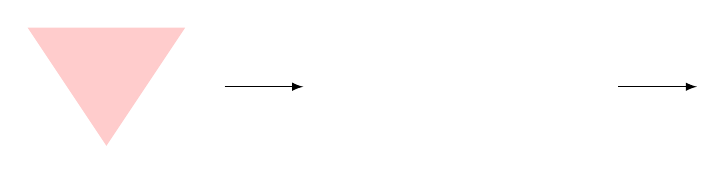
\begin{tikzpicture}
      \fill[opacity = 0.2, red] (2, 0) -- (1, 1.5) -- ( 3, 1.5) -- cycle; 
      \Vertex[x=0, y=0, size=0.25, fontscale=0.75, label=1]{v1}
      \Vertex[x=2, y=0, size=0.25, fontscale=0.75,label=2]{v2}
      \Vertex[x=1, y=1.5, size=0.25,fontscale=0.75, label=3]{v3}
      \Vertex[x=3, y=1.5, size=0.25,fontscale=0.75, label=4]{v4}
      \Edge(v1)(v2)
      \Edge(v1)(v3)
      \Edge(v2)(v3)
      \Edge(v2)(v4)
      \Edge(v3)(v4)

      \draw[-latex] ( 3.5, 0.75) -- (4.5, 0.75) ;

      \Vertex[x=5, y=0, size=0.25, fontscale=0.75, label=1]{v1}
      \Vertex[x=7, y=0, size=0.25, fontscale=0.75,label=2]{v2}
      \Vertex[x=6, y=1.5, size=0.25,fontscale=0.75, label=3]{v3}
      \Vertex[x=8, y=1.5, size=0.25,fontscale=0.75, label=4]{v4}
      \Edge(v1)(v2)
      \Edge(v1)(v3)
      \Edge(v2)(v3)
      \Edge(v2)(v4)

      \draw[-latex] ( 8.5, 0.75) -- (9.5, 0.75) ;

      \Vertex[x=10, y=0, size=0.25, fontscale=0.75, label=1]{v1}
      \Vertex[x=12, y=0, size=0.25, fontscale=0.75,label=2]{v2}
      \Vertex[x=11, y=1.5, size=0.25,fontscale=0.75, label=3]{v3}
      \Edge(v1)(v2)
      \Edge(v1)(v3)
      \Edge(v2)(v3)

\end{tikzpicture}}{Example of weakly collapsible but not collapsible simplicial complex \label{fig:weak_example}}
\end{example}

\begin{theorem}\label{thm:poly}
      Weak collapsibility of \( 2\)-skeleton \( \mc K \) is polynomially solvable.
\end{theorem}
\begin{proof}
      The \emph{greedy algorithm} for the collapsing sequence intuitively operates as follows: at each iteration perform any of possible collapses; in the absence of free edges, the complex should be considered not collapsible, \Cref{algo:greedy}. Clearly, such an algorithm runs polynomially with respect to the number of simplexes in \(\mc K\).
      % TODO:

      The failure of the greedy algorithm indicates the existence of a weakly collapsible complex \( \mc K \) such that the greedy algorithm gets stuck at a \( 2 \)-Core, which is avoidable for another possible order of collapses. Among all the counter exemplary complexes, let \( \mc K \) be a minimal one with respect to the number of triangles \( m_2 \). Then there exist a free edge \( \sigma \in \V 1 \) such that \( \mc K \backslash \{ \sigma \} \) is \emph{collapsible} and another \( \sigma' \in \V 2 \) such that \( \mc K \backslash \{ \sigma' \} \) is \emph{not collapsible}.

      Note that if \( \mc K \) is minimal then for any pair of free edges \( \sigma_1 \) and \( \sigma_2 \) belong to the same triangle: \( \tau(\sigma_1) = \tau(\sigma_2) \). Indeed, for any \( \tau(\sigma_1) \ne \tau(\sigma_2) \),  \( \mc K \backslash \{ \sigma_1, \sigma_2 \} = \mc K \backslash \{ \sigma_2, \sigma_1 \} \). Let \( \tau(\sigma_1) \ne \tau(\sigma_2) \) for at least one pair of \( \sigma_1 \) and \( \sigma_2 \); in our assumption, either both \( \mc K \backslash \{ \sigma_1 \} \) and \( \mc K \backslash \{ \sigma_2 \} \), only \( \mc K \backslash \{ \sigma_1 \}  \) or none are collapsible. In the former case either \( \mc K \backslash \{ \sigma_1 \} \) or \( \mc K \backslash \{ \sigma_2 \} \) is a smaller example of the complex satisfying the assumption, hence, violating the minimality. If only \( \mc K \backslash \{ \sigma_1 \} \) is collapsible, then \( \mc K \backslash \{ \sigma_2, \sigma_1 \}  \) is not collapsible; hence, \( \mc K \backslash \{ \sigma_1, \sigma_2 \} \) is not collapsible, so \( \mc K \backslash \{ \sigma_1 \} \) is a smaller example of a complex satisfying the assumption. Finally, if both \( \mc K \backslash \{ \sigma_1 \} \) and \( \mc K \backslash \{ \sigma_2 \} \) are collapsible, then for  known \( \sigma' \) such that \( \mc K \backslash \{ \sigma' \} \) is not collapsible, \( \tau(\sigma') \ne \tau(\sigma_1)\) or \( \tau(\sigma') \ne \tau(\sigma_2) \), which revisits the previous point.

      As a result, for \( \sigma \) ( \( \mc K \backslash \{ \sigma \} \) is collapsible) and for \( \sigma' \) ( \( \mc K \backslash \{ \sigma' \} \) is not collapsible ) it holds that \( \tau (\sigma) = \tau (\sigma') \Rightarrow  \sigma \cap \sigma' = \{ v \}  \), so after collapses \( \mc K  \{ \sigma \} \) and \( \mc K \backslash \{ \sigma' \} \) we arrive at two identical simplicial complexes modulo the hanging vertex irrelevant for the weak collapsibility. A simplicial complex can not be simultaneously collapsible and not collapsible, so the question of weak collapsibility can always be resolved by the greedy algorithm which has polynomial complexity.
\end{proof}

\begin{comment}
\blav
\begin{remark}
      The proof above is reminiscent of the one for polynomiality of \(d\)-collapsibility, \( d = 1\) or \( d = 2\), \cite{tancer2008dcollapse}, but bares significant differences: firstly, \( 2 \)-collapsibility allows collapses at \(\sigma: \; \dim \sigma \le 1\); secondly, in the scope of \cite{tancer2008dcollapse}, \( \tau(\sigma) = \sigma \) is allowed which affects (complicates) the proof.
\end{remark}
\elav


\begin{remark}
      If \( \mc K \) is weakly collapsible, then the number of triangles can not be higher than the number of edges, \( m_2 \le m_1 \), hence \( \mc K \) is \emph{necessarily sparse} and does not breach the gap up to \( m_2 = \mc O\left( m_1 \ln \left( 4 m_1 \right) \right) \).
\end{remark}
\end{comment}

\subsection{Computational cost of the greedy algorithm}

Let \( \mc K \) be a \(2\)-skeleton; let \( \Delta_\sigma \) be a set of triangles of \( \mc K \) containing the edge \( \sigma \), \( \Delta_\sigma = \{ t \mid  t \in \V 2  \text{ and } \sigma \in t \} \). Then the edge \( \sigma \) is free iff \( | \Delta_\sigma | = 1 \) and \( F = \{ \sigma \mid | \Delta_e | = 1  \} \) is a set of all free edges. Note that \( | \Delta_e | \le m_0 -2 = \mc O ( m_0  ) \).

\begin{algorithm}[h]
      \caption{ \texttt{GREEDY\_COLLAPSE}(\(\mc K\)):  greedy algorithm for the weak collapsibility
      \label{algo:greedy}}
      \begin{algorithmic}[1]
            \Require initial set of free edges \( F \), adjacency sets \(  \{ \Delta_{ \sigma_i } \}_{i=1}^{ m_1 } \)
             \State \( \Sigma = [ \; ] , \; \ds T = [ \; ] \) \Comment{ initialize the collapsing sequence}
             \While{ \( F \ne \vn \) \textbf{ and } \( \V 2 \ne \vn \) }
                  \State \( \sigma \gets \texttt{pop}( F ) \), \( \; \tau \gets \tau(\sigma)  \) \Comment{ pick a free edge \( \sigma \) }
                  \State \( \mc K \gets \mc K \backslash \{ \sigma \} \), \( \; \Sigma \gets [ \, \Sigma \;\; \sigma \, ] , \; \ds T \gets [ \ds T \; \tau ] \) \Comment{ \small \( \tau \) is a triangle being collapsed; \( \tau = [ \sigma, \sigma_1, \sigma_2 ] \) }
                  \State \( \Delta_{\sigma_1} \gets \Delta_{\sigma_1} \backslash \tau  \), \( \; \Delta_{\sigma_2} \gets \Delta_{\sigma_2} \backslash \tau  \) \Comment{ remove \( \tau \) from adjacency lists }
                  \State \( F \gets F \cup \{ \sigma_i \, |  \, i = 1, 2 \text{ and } | \Delta_{\sigma_i} | = 1 \}  \) \Comment{ update \( F \) if any of \( \sigma_1 \) or \( \sigma_2 \) has become free }
                  %\State \( \mc K \gets \mc K  \backslash \{ \sigma \} \) \Comment{ perform a collapse  }
             \EndWhile
             \State \Return \( \mc K, \, \Sigma, \, \ds T \)
      \end{algorithmic}
\end{algorithm}

The complexity of \Cref{algo:greedy} rests upon the precomputed \( \sigma \mapsto \Delta_\sigma \) structure that de-facto coincides with the boundary operator \( B_2 \) (assuming \( B_2 \) is stored as a sparse matrix, the adjacency structure describes its non-zero entries). Similarly, the initial \( F \) set can be computed alongside the construction of \( B_2 \) matrix. Another concession is needed for the complexity of the removal of elements from \( \Delta_{\sigma_i} \) and \( F \), which may vary from \( \mc O (1) \) on average up to guaranteed \( \log ( | \Delta_{\sigma_i} | ) \). As a result, given a pre-existing \( B_2 \) operator, \Cref{algo:greedy} runs linearly, \( \mc O ( m_1  )\), or almost linearly depending on the realisation, \( \mc O ( m_1 \log m_1 )\).








